\hypertarget{a00366}{}\section{D\+T\+T Guide}
\label{a00366}\index{D\+T\+T Guide@{D\+T\+T Guide}}
How to automate different test scenarios for D\+S\+H. 

\hypertarget{a00366_dtt_guide_contents}{}\subsection{Contents}\label{a00366_dtt_guide_contents}
\begin{DoxyItemize}
\item \hyperlink{a00366_dtt_guide_00_what_is_dtt}{What is D\+T\+T} \item \hyperlink{a00366_dtt_guide_01_how_to_run_test_and_suites_in_dtt}{How to run tests and suites in D\+T\+T} \item \hyperlink{a00366_dtt_guide_03_writing_dtt_scripts}{Writing D\+T\+T scripts} \item \hyperlink{a00366_dtt_guide_04_logging_in_dtt_and_debuggin_dtt_scripts}{Logging in D\+T\+T and debugging D\+T\+T scripts} \item \hyperlink{a00366_dtt_guide_02_working_with_dtt_test_suites}{Working with D\+T\+T test suites}\end{DoxyItemize}
 \hypertarget{a00366_dtt_guide_00_what_is_dtt}{}\subsection{What is D\+T\+T}\label{a00366_dtt_guide_00_what_is_dtt}
 Dish\+Test\+Tool (D\+T\+T) is a Ruby-\/based command line tool, which provides the ability to script and thus automate D\+S\+H test scenarios. It is included in the Digi\+Shell Tools package in the /\+D\+T\+T directory.

\begin{DoxyNote}{Note}
Ruby is installed by default on O\+S X. On Windows, you will need to install Ruby and add it to your P\+A\+T\+H variable manually. For information regarding Ruby version compatibility with a specific build of D\+T\+T, see the Read\+Me.\+txt file in /\+D\+T\+T/sources.
\end{DoxyNote}
The D\+T\+T folder consists of\+: 
\begin{DoxyItemize}
\item {\itshape Sources} 
\begin{DoxyItemize}
\item D\+T\+T core 
\item {\itshape scripts} folder -\/ place all D\+T\+T script files here

By default, this folder includes a few example scripts demonstrating basic D\+T\+T operations and plug-\/in testing steps\+:


\begin{DoxyItemize}
\item {\itshape D\+S\+H\+\_\+\+Sig\+Cancellation.\+rb} -\/ script for the cancellation test  
\item {\itshape D\+S\+H\+\_\+\+T\+I\+\_\+\+Cycle\+Counts} -\/ script for performing cycle count test 
\item {\itshape Suite\+Generator.\+rb} -\/ generates suites for the D\+S\+H\+\_\+\+Sig\+Cancellation and D\+S\+H\+\_\+\+T\+I\+\_\+\+Cycle\+Counts tests 
\end{DoxyItemize}
\item {\itshape suites} folder -\/ place your D\+T\+T suite files here 
\end{DoxyItemize}
\item {\itshape run\+\_\+test.\+command} (on Mac) or {\itshape run\+\_\+test.\+bat} (on Windows) -\/ command file for runnung tests 
\item {\itshape run\+\_\+irb.\+command} (on Mac) or {\itshape run\+\_\+irb.\+bat} (on Windows) -\/ command-\/line interpreter 
\end{DoxyItemize}

 \hypertarget{a00366_dtt_guide_01_how_to_run_test_and_suites_in_dtt}{}\subsection{How to run tests and suites in D\+T\+T}\label{a00366_dtt_guide_01_how_to_run_test_and_suites_in_dtt}
 {\ttfamily run\+\_\+test} is the main D\+T\+T execution program. {\ttfamily run\+\_\+test} is able to execute Ruby scripts which have been placed in the scripts folder within the D\+T\+T directory.


\begin{DoxyItemize}
\item {\ttfamily run\+\_\+test.\+command -\/l} -\/ lists all the available scripts and suites 
\item {\ttfamily run\+\_\+test.\+command 1} -\/ runs test by number 
\item {\ttfamily run\+\_\+test.\+command D\+S\+H\+\_\+\+Sig\+Cancellation} -\/ runs a test by name. Pay attensions that the name of test should be without (!) extension. 
\item {\ttfamily run\+\_\+test.\+command --script D\+S\+H\+\_\+\+Sig\+Cancellation -\/a sample\+\_\+rate=48000 -\/a threshold=-\/80} -\/ runs a test with test script arguments, which are specified using the {\ttfamily -\/a} option 
\end{DoxyItemize}

 Figure 1\+: running D\+T\+T tests.

For more information about script arguments, see \hyperlink{a00366_describing_and_using_input_arguments_of_the_script}{Describing and using input arguments of the script}



 \hypertarget{a00366_dtt_guide_03_writing_dtt_scripts}{}\subsection{Writing D\+T\+T scripts}\label{a00366_dtt_guide_03_writing_dtt_scripts}
 Most of the D\+T\+T scripts require {\ttfamily Digi\+Shell}, which allows them to run dsh and execute different dsh commands. Each script should be represented in the form of class, which inherits Script class, and also each script must have at least two elements\+: self.\+inputs section, where all the input arguments of the test should be described, and run method, which is the main body of your script.


\begin{DoxyCode}
require \textcolor{stringliteral}{'DigiShell'}

\textcolor{keyword}{class }ScriptSample < Script
   def self.inputs
      return \{\}
   end

   def run
      \textcolor{keywordflow}{return} pass(\textcolor{stringliteral}{"Well, it didn't explode.  So that's something."});
   end
end
\end{DoxyCode}
 Listing 1\+: Skeleton of the script

\hypertarget{a00366_describing_and_using_input_arguments_of_the_script}{}\subsubsection{Describing and using input arguments of the script}\label{a00366_describing_and_using_input_arguments_of_the_script}
 The available parameters and their values for a script are listed in the static {\ttfamily self.\+inputs} routine. Input arguments must be organized in the form of a hash map which is returned from this routine.


\begin{DoxyCode}
def \textcolor{keyword}{self}.inputs
    \textcolor{keywordflow}{return} \{
      :sample\_rate     => [44100,[44100,48000,88200]],
      :path\_to\_tfx     => [\textcolor{stringliteral}{'none'}],
      :threshold       => [-96],
    \}
end

@dsh.init\_dae(sample\_rate)
\end{DoxyCode}
 Listing 2\+: Desribing input arguments for the script and using them

Hash entries should be in the following format\+:  \+:arg\+\_\+name =$>$ \mbox{[}default\+\_\+value, \mbox{[}range of allowed values\mbox{]}\mbox{]} 

These arguments can be used then by just calling them by name, like in the example above with {\ttfamily sample\+\_\+rate} argument.

\hypertarget{a00366_writing_body_of_the_script}{}\subsubsection{Writing body of the script}\label{a00366_writing_body_of_the_script}
 The body of the script must be enclosed in the body of the {\ttfamily run} method of the script class. As far as most D\+T\+T tests need D\+S\+H, in the example below it\textquotesingle{}s shows how to create a D\+S\+H instance in the script and how to use it then. D\+S\+H instance can be creted with {\ttfamily Digi\+Dhell.\+new} method, which requites Digi\+Shell module, as has already been said. Then all the D\+S\+H commands become available as methods of the D\+S\+H instance, and input arguments can be passed to these command as input arguments for the methods, i.\+e. in parentheses {\ttfamily dsh.\+load\+\_\+dish(\char`\"{}\+D\+A\+E\char`\"{})}. Also it\textquotesingle{}s recommended to handle possible exceptions that may occure during the execution of the code, and to make sure that D\+S\+H has been closed, if it was instantiated on the moment of the failure.


\begin{DoxyCode}
def run
   begin
      dsh = DigiShell.new(target)
      dsh.load\_dish(\textcolor{stringliteral}{"DAE"})
      dsh.init\_dae(sample\_rate)
      dsh.close

      \textcolor{keywordflow}{return} pass(\textcolor{stringliteral}{"Well, it didn't explode.  So that's something."})

   rescue Exception => e
      \textcolor{preprocessor}{# make sure to close down dsh before returning}
      \textcolor{keywordflow}{if} (dsh)
         dsh.close
      end
        
      \textcolor{keywordflow}{return} fail(e)
   end
end
\end{DoxyCode}
 Listing 3\+: Example of the body of the script.



 \hypertarget{a00366_dtt_guide_04_logging_in_dtt_and_debuggin_dtt_scripts}{}\subsection{Logging in D\+T\+T and debugging D\+T\+T scripts}\label{a00366_dtt_guide_04_logging_in_dtt_and_debuggin_dtt_scripts}
 D\+T\+T tool has logging, and all the logs collected in the Logs folder, which is located in root directory of the D\+T\+T. D\+T\+T creates a separate folder for each test and names these folders with the corresponding names + the time when the particular test has been executed. For example\+:

{\ttfamily D\+S\+H\+\_\+\+Sig\+Cancellation\+\_\+20131225\+\_\+185146\+\_\+0001}

Inside each folder there are several log files\+: 
\begin{DoxyItemize}
\item {\itshape xxx.\+html} – contains info about input \& output of the test in a fancy form (tables) 
\item {\itshape xxx\+\_\+c.\+txt} – contains the list of the D\+S\+H commands that have been executed 
\item {\itshape xxx\+\_\+d.\+txt} – D\+S\+H output 
\item {\itshape xxx\+\_\+i.\+txt} – info about your system 
\item {\itshape xxx\+\_\+l.\+txt} – standard output 
\item {\itshape xxx\+\_\+v.\+txt} – verbose output 
\end{DoxyItemize}

\hypertarget{a00366_dtt_guide_04_interactive_mode}{}\subsubsection{Interactive mode}\label{a00366_dtt_guide_04_interactive_mode}
 There is an option to run D\+T\+T in interactive mode using interactive ruby shell (irb). When running in this mode, D\+T\+T creates a shell which is an extended version of the standard Ruby interpreter. Besides the standard functionality, it knows how to work with D\+T\+T classes and can give hints on their methods. In particular, the D\+T\+T interactive mode shell knows how to work with Digi\+Shell.

To run D\+T\+T in interactive mode, go to the D\+T\+T folder and launch the {\ttfamily run\+\_\+irb} program. At this point you will send ruby commands to dsh through the pipe in Y\+A\+M\+L format\+:


\begin{DoxyCode}
t = Target.new # creates an instance of Target. In \textcolor{keyword}{this} \textcolor{keywordflow}{case} target is a local machine, though we have a 
      possibility to run test on remote machine.
dsh = DigiShell.new(t) # creates an instance of DigiShell(aka launching dsh binary)
dsh.load\_dish(\textcolor{stringliteral}{'DAE'}) #Loads \textcolor{stringliteral}{'DAE'} dish
dsh.help(\textcolor{stringliteral}{'init\_dae'}) # Requests help from dsh \textcolor{keywordflow}{for} \textcolor{stringliteral}{'init\_dae'} command
dsh.init\_dae
plugins = dsh.run #returns an array of plug-ins and writes them to plugins var.
plug-ins[0] #reaching first plug-in from the list
\textcolor{preprocessor}{#... whatever you want to do}
\end{DoxyCode}
 Listing 4\+: Running D\+T\+T in interactive mode



 \hypertarget{a00366_dtt_guide_02_working_with_dtt_test_suites}{}\subsection{Working with D\+T\+T test suites}\label{a00366_dtt_guide_02_working_with_dtt_test_suites}
 Suites are files which contain the list of D\+T\+T scripts that should be run, and parameteres for these tests. These files should be created in Y\+A\+M\+L format. The list of the tests should be preceeded by {\ttfamily tests\+:} line. Then tests to be run should be described as a map with the following members\+:


\begin{DoxyItemize}
\item {\ttfamily name\+: } -\/ name of the test 
\item {\ttfamily enabled\+: } -\/ determines whether test will be run or skipped 
\item {\ttfamily args\+: } -\/ input parameters of the test 
\end{DoxyItemize}

The input parameters of the test should be orginized as a hash map. That means that all keys should start with \char`\"{}\+:\char`\"{} and look like \char`\"{}\+:plugin\+\_\+spec\+: \char`\"{}.

Also suite may contain a section with the general parameters like\+:


\begin{DoxyItemize}
\item {\ttfamily verbose\+: false} which determines whether the output of the test in the console will be verbose or not. 
\item {\ttfamily timeout\+Factor\+: \char`\"{}16.\+0\char`\"{}} which defines the time period, after which test will exit in case it stuck on the execution of the certain peice of code. 
\end{DoxyItemize}

Example of the suite\+: 
\begin{DoxyCode}
suitesettings:
  verbose: \textcolor{keyword}{false} 
tests: 
\textcolor{preprocessor}{#}
\textcolor{preprocessor}{# Cycle counting test}
\textcolor{preprocessor}{#}
- name: DSH\_TI\_CycleCounts 
  enabled: \textcolor{keyword}{true} 
  args: 
    :plugin\_spec: \textcolor{stringliteral}{'Digi,Pich,Psmm'} 
    :sample\_rate: 48000
\end{DoxyCode}
 Listing 5\+: Example of the D\+T\+T test suite

\begin{DoxyNote}{Note}
All the suites files should have an extension .gss
\end{DoxyNote}
\hypertarget{a00366_autogeneration_of_the_suites}{}\subsubsection{Autogeneration of the suites}\label{a00366_autogeneration_of_the_suites}
 Sometimes it is necessary to generate the suites for the particular script for all the plug-\/ins from the bundle and/or for different sample rates. In this case instead of the copy-\/paste, which may lead to some mistakes and erratums, suitegenerator can be used. This is a special script, which takes as arguments the name of the script(s), for which the suites should be generated, and the list of their input parameters. Strange as it may sound, this data should be formed as a suite. Script itself is available as Suite\+Generator.\+rb along with other scripts in the D\+T\+T.

\begin{DoxyNote}{Note}
Suite\+Generator.\+rb can generate suites only for the two tests\+: D\+S\+H\+\_\+\+Sig\+Cancellation test and D\+S\+H\+\_\+\+T\+I\+\_\+\+Cycle\+Counts test
\end{DoxyNote}
Here is the example of how to use this script to generate the suites for all the plug-\/ins from the \textquotesingle{}D-\/\+Verb\textquotesingle{} bundle for all the sample rates the cancellation test A\+A\+X Native vs A\+A\+X D\+S\+P, and for the cycle counts test\+:


\begin{DoxyCode}
tests:
\textcolor{preprocessor}{# Generate suite for Cancellation test: AAX Native vs AAX DSP}
- name: SuiteGenerator
  args: 
    :plugin\_name: \textcolor{stringliteral}{'D-Verb'}
    :path\_to\_audio\_files: /Volumes/G\_Audio/GS\_Test\_Resources/audio/
    :path\_to\_presets: /Volumes/G\_Audio/GS\_Test\_Resources/PL\_Settings/
    :test\_script: DSH\_SigCancellation
  enabled: \textcolor{keyword}{true}
\textcolor{preprocessor}{# Generate suite for Instance Count test}
- name: SuiteGenerator
  args: 
    :plugin\_name: \textcolor{stringliteral}{'D-Verb'}
    :path\_to\_presets: /Volumes/G\_Audio/GS\_Test\_Resources/PL\_Settings/
    :test\_script: DSH\_TI\_CycleCounts\_se
  enabled: \textcolor{keyword}{true}
suitesettings: 
  verbose: \textcolor{keyword}{false}
  timeoutFactor: \textcolor{stringliteral}{"16.0"}
\end{DoxyCode}
 Listing 6\+: Example of how to use Suite\+Generator script for generating suites for all the plug-\/ins from the \textquotesingle{}D-\/\+Verb\textquotesingle{} bundle for the all sample rates for the cancellation and for the cycle counts test.

To generate the suites, one should run this suite for the Suite\+Generator as an ordinary suite by executing the {\ttfamily run\+\_\+test.\+command $<$the name of the suite for the Suite\+Generator$>$} command. All the suites will be generated into the single file, which will be located inside the suites folder, and will be called like\+:

{\ttfamily dsp\+V\+Snative(optional)\+\_\+$<$the name of the plug-\/in$>$\+\_\+$<$the name of the test$>$.gss}

Examples\+: 
\begin{DoxyItemize}
\item T\+R\+I\+M\+\_\+\+D\+S\+H\+\_\+\+T\+I\+\_\+\+Cycle\+Counts.\+gss 
\item dsp\+V\+Snative\+\_\+\+T\+R\+I\+M\+\_\+\+D\+S\+H\+\_\+\+Sig\+Cancellation.\+gss 
\end{DoxyItemize}

 Collaboration diagram for D\+T\+T Guide\+:
\nopagebreak
\begin{figure}[H]
\begin{center}
\leavevmode
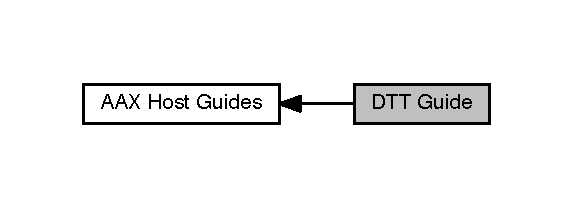
\includegraphics[width=275pt]{a00366}
\end{center}
\end{figure}
